\chapter{Especificación semántica}
\section{Introducción}
El objetivo de este capítulo es realizar la especificación semántica del lenguaje y mostrar un pseudocódigo de su implementación.

Para llevar acabo la especificación semántica, trabajaremos sobre el analizador sintáctico de la sección anterior, realizando modificaciones que permitan implementar el analizador semántico.% utilizando una Definición Dirigida por la Sintaxis .

\section{Descripción del problema}
\label{sec:sem:descr_probl}
En esta etapa del desarrollo del compilador necesitamos extender el analizador sintáctico para poder realizar verificaciones semánticas sobre el programa a compilar. Los chequeos semánticos a realizar son:
\begin{itemize}
\item Existencia: los identificadores utilizados en el cuerpo del programa deben estar previamente declarados. El alcance de los identificadores es estático, por lo que un identificador no declarado en un ambiente se buscará en sus ambientes ancestros.
\item Unicidad: no se permite tener más de un identificador con el mismo nombre declarado en un mismo ambiente.
\item Correspondencia de parámetros: la llamada a procedimientos o funciones debe coincidir con la signatura del procedimiento o la función invocada.
\item Compatibilidad y equivalencia de tipos: los operandos de un operador deben ser compatibles para poder ejecutar correctamente la operación. %Se hará la coerción necesaria donde sea adecuado.
\end{itemize}

\section{Compatibilidad de tipos}
En la tabla \ref{tab:compatibilidad} se muestra cada operador, los tipos de los operandos que puede recibir y el tipo de resultado de la operación.

El operador ``-'' es el único operador sobrecargado, ya que puede ser utilizado tanto para operaciones binarias como unarias. En el caso de usarlo como operación unaria, su tipo de operando y resultado es el mismo que para la operación binaria. 
\begin{table}[H]
\centering
\begin{tabular}{|c|c|c|c|}
\hline
Operador                                                & Operando 1      & Operando 2      & Resultado \\ \hline
+, -,*,/                                                & Integer         & Integer         & Integer   \\ \hline
=, \textless{}\textgreater{}                            & Integer/Boolean & Integer/Boolean & Boolean   \\ \hline
\textless{},\textless{}=,\textgreater{},\textgreater{}= & Integer         & Integer         & Boolean   \\ \hline
and, or                                                 & Boolean         & Boolean         & Boolean   \\ \hline
not                                                     & Boolean         & -               & Boolean   \\ \hline
:=                                                      & Boolean         & Boolean         & -         \\ \hline
:=                                                      & Integer         & Integer         & -         \\ \hline
\end{tabular}
\caption{Compatibilidad de tipos}
\label{tab:compatibilidad}
\end{table}

\section{Estrategias}
Se utilizaron estructuras de objetos para la representación de la tabla de símbolos de manera que esta fuera fácilmente accedida por el Analizador Semántico. En tal estructura se dispusieron atributos de manera que se pueda identificar el nombre del programa, función o procedimiento que corresponde al ambiente nuevo, como también listas para los tipos de los identificadores reconocidos en su interior, y para los parámetros que recibe, en caso de que corresponda. Esto nos permitió chequear fácilmente el retorno de las funciones y las llamadas recursivas, los cuales son casos particulares que deben tratarse.

%\section{Limitaciones}
%La estructura desarrollada para la tabla de símbolos presenta limitaciones con respecto a la expansión de los atributos que esta puede almacenar para cada identificador. Esto es debido a que se plantearon como listas de atributos solo aquellas características que se deseaban almacenar para los chequeos que se proponen en la sección \ref{sec:sem:descr_probl}. Por lo tanto si se desean agregar mas atributos, es necesario agregar nuevas listas en la estructura, donde se mapeen los identificadores a su valor de atributo, como también sus métodos de acceso correspondientes. Por ejemplo para almacenar el valor de los tipos de los identificadores en la tabla de símbolos, se utiliza una lista que mapea de identificadores a tipos, y se deben agregar todas las operaciones correspondientes para acceder a esta lista. En este sentido, el acceso a los datos de la tabla de símbolos no es genérico ya que si quiero acceder a otro dato, como los parámetros de un subprograma, debo utilizar otra operación correspondiente para tal acceso.

%esto no es una limitación, es una característica de la implementación de la TS. Desde el punto de vista del semántico la tabla de símbolos es genérica porque le provee las operaciones que necesita el semántico.

\section{Diseño del analizador semántico}
Para modelar el diseño del analizador semántico, se trabajará sobre algunas reglas de la gramática de la sección \ref{sec:gramatica_mod}, agregando acciones semánticas. Estas acciones permiten extender la potencia de las gramáticas libres de contexto, convirtiendo la gramática en una gramática de atributos.

Toda aquella información que se requiera persistir para las acciones semánticas, y que no pueda ser enviada mediante parámetros entre las llamadas de las reglas de la gramática, será almacenada en la tabla de símbolos para su posterior acceso.

\subsection{Tabla de símbolos}
La tabla de símbolos (TS) es la estructura que guarda toda la información necesaria para el proceso de análisis semántico. En este trabajo, proponemos una tabla de símbolo para cada ambiente particular.
Como el alcance de los identificadores es estático, cada identificador pertenecerá a un ambiente \emph{A}, y podrá ser accedido por aquellos ambientes \emph{A'} que estén contenidos en \emph{A}.

El Analizador Semántico mantendrá siempre una referencia a la Tabla de Símbolos del ambiente actual que esté procesando.

En la Tabla \ref{tab:tabla_simbolos} se esquematiza la forma que tendrá la tabla de símbolos explicada.

\begin{table}[H]
	\centering
	\begin{tabular}{|c|c|c|c|c|c|}
		\hline
		Ambiente & Nombre & Tipo & \multicolumn{3}{c|}{Listas de valores} \\ \hline
		\multirow{5}{*}{1} & \multirow{5}{*}{$ambiente_1$} & \multirow{5}{*}{\begin{tabular}[c]{@{}c@{}}{[}program $\lvert$ \\ function $\lvert$ \\ procedure{]}\end{tabular}} & Identificador & Tipo & Parámetros \\ \cline{4-6} 
		&  &  & $id_{var}$ & \begin{tabular}[c]{@{}c@{}}{[}integer $\lvert$ \\ boolean{]}\end{tabular} & {[} {]} \\ \cline{4-6} 
		&  &  & $id_{subprogram}$ & void & {[} $param_1$, \dots, $param_n$ {]} \\ \cline{4-6} 
		&  &  & \multicolumn{3}{c|}{\dots} \\ \cline{4-6} 
		&  &  & $id_n$ & \dots & \dots \\ \hline
		\multicolumn{6}{|c|}{\dots} \\ \hline
		n & $ambiente_n$ & \dots & \dots & \dots & \dots \\ \hline
	\end{tabular}
\caption{Esquema de la tabla de símbolos diseñada.}
\label{tab:tabla_simbolos}
\end{table}

\subsection{Gramática de atributos}
\label{sec:sem:gram_atrib}
Algunas reglas de la gramática serán alteradas para insertar y recuperar información de la tabla de símbolos, y permitirán cumplir con los objetivos propuestos en la sección \ref{sec:sem:descr_probl}.
Los siguientes no terminales se verán modificados, y sus correspondientes implementaciones en el Analizador Sintáctico cambiarán según estas modificaciones:

\begin{itemize}
\item $<$bool$>$ sintetiza el atributo \texttt{type} indicando el type boolean.
\item $<$number$>$ sintetiza el atributo \texttt{type} indicando el type integer.
\item $<$literal$>$ sintetiza el atributo \texttt{type} con el type del literal. Este valor se extrae del atributo sintetizado de $<$bool$>$ o $<$number$>$.
\item $<$factor$>$ sintetiza el atributo \texttt{type}. También verifica que pueda aplicarse el operador unario correctamente en $<$factor$>$ $\rightarrow$ $<$factor$_1$$>$ utilizando el atributo \texttt{type} de $<$factor$_1$$>$.
\item $<$identifier$>$ sintetiza el atributo \text{id} con el valor del identificador.
\item $<$type$>$ sintetiza el atributo \texttt{type} indicando el valor del tipo de dato. 
\item $<$expression-or$>$, $<$expression-and$>$, $<$expression-rel$>$, $<$expression-add$>$, $<$expression-mult$>$ y $<$factor$>$ sintetizan el atributo \texttt{type} que indica el tipo dato de la expresión.
\item $<$expression-or$_1>$, $<$expression-and$_1>$, $<$expression-rel$_1>$, $<$expression-add$_1>$, $<$expression-mult$_1>$ verifican que pueda aplicarse su operación correspondiente usando el atributo \texttt{type1} sintetizado y \texttt{type2} heredado . 
\item $<$identifier-list$>$ sintetiza el atributo \texttt{list\_id} que devuelve una lista de identificadores. Para cargar la lista utiliza el atributo sintetizado \texttt{id} de $<$identifier$>$.
\item $<$variable-declaration$>$ utiliza los atributos sintetizados \texttt{list\_id} y \texttt{type} para insertar en la tabla de símbolos cada identificador con su tipo.
\item $<$parameter-declaration$>$ sintetiza un atributo \texttt{list\_parameters} que devuelve una lista con listas de identificadores y sus tipos.
\item $<$procedure-heading$>$ utiliza el atributo sintetizado \texttt{id} y lo guarda en la tabla de simbolos. También utiliza el atributo sintetizado de $<$parameter-declaration$>$ para guardar los parámetros y sus tipos en la tabla de símbolos
\item $<$function-heading$>$ utiliza los atributos sintetizados \texttt{id} y \texttt{type} y los guarda en la tabla de símbolos. También utiliza el atributo sintetizado de $<$parameter-declaration$>$ para guardar los parámetros y sus tipos en la tabla de símbolos
\item $<$assignment-statement$>$ utiliza el atributo heredado \texttt{type} junto con el atributo sintetizado \texttt{type} de $<$expression-or$>$ para verificar si se puede efectuar la asignación.
\item $<$conditional-statement$>$ y $<$repetitive-statement$>$ utilizan el atributo sintetizado \texttt{type} de $<$expression-or$>$ para verificar que la expresión de la condición sea booleana.
\end{itemize}

\section{Implementación del aplicativo}
En esta sección mostraremos las principales modificaciones del analizador sintáctico teniendo en cuenta la gramática \ref{sec:sem:gram_atrib}. 

\subsection{Descripción del problema}
En esta etapa se requiere implementar el Analizador Semántico. Como es un análisis que debe hacerse en conjunto con el análisis sintáctico, el código del Analizador Semántico será embebido en el Analizador Sintáctico.

Cuando se encuentre un error semántico, se lanzará un error que brinde información significativa para poder corregirlo. 

\subsection{Herramientas utilizadas}
Para desarrollar el programa continuamos desde el mismo proyecto que el Analizador Sintáctico, en lenguaje Java. La versión de Java sobre la que trabajamos es la 8\footnote{Actualización 171, al día 14/05/2018}(ocho), sobre el sistema operativo Windows 10. 

\subsection{Diseño}
La idea del Analizador Semántico es modificar los procedimientos implementados del Analizador Sintáctico. Cuando un procedimiento requiera acceder a atributos sintetizados, creará variables para poder recibir los atributos; y cuando un procedimiento requiera atributos heredados, los recibirá por parámetro. 

Para no perder la implementación del Analizador Sintáctico, crearemos otra clase llamada \textbf{AnalizadorSemántico} dentro del paquete \textbf{semantico} con el mismo código del \textbf{AnalizadorSintactico}, y además crearemos el TDA \textbf{Ambiente}, por lo que nuestro árbol de directorios quedará como en la figura \ref{fig:arbol_dir_4}.

\begin{figure}[H]
%no borrar el % de dirtree porque es necesario.
\dirtree{%
.1 src.
.2 compiladorpascal.
.3 CompiladorPascal.java.
.3 lexico.
.3 sintactico.
.3 semantico.
.4 AnalizadorSemantico.java.
.4 Ambiente.java.
}
\caption{Árbol de directorios del proyecto de Java con los archivos del analizador semántico.}
\label{fig:arbol_dir_4}
\end{figure}

Para manejar los errores, creamos los métodos \texttt{errorSemantico()} y \texttt{errorSintactico()}, para que sea más fácil la invocación de errores, y se puedan mostrar mensajes adecuados.

El diseño de la tabla de símbolos se basa en guardar todo el contenido de un ambiente en su respectiva instancia del TDA \textbf{Ambiente}. Para cada ambiente del programa se guardan sus identificadores. Si el identificador es una variable o una función se le asigna su tipo, en el caso de los procedimientos se les asigna el tipo \texttt{void} por defecto. Si el identificador es una función o procedimiento, se le asocia una lista que contiene los tipos de sus parámetros manteniendo el orden en el que son declarados.

Cuando inicia el programa se crea el ambiente principal, y luego cada vez que se inicia una función o un procedimiento se crea un ambiente nuevo y se asigna como padre de este al ambiente anterior. Cuando se termina de analizar el cuerpo de un procedimiento o función, se actualiza la referencia del analizador semántico con el padre del ambiente analizado.

A continuación podemos ver la interfaz de la clase \textbf{Ambiente}.

\begin{minted}[autogobble,linenos,xleftmargin=0.025\textwidth,xrightmargin=0.025\textwidth,breaklines]{java}
public class Ambiente {
	Ambiente padre; //ambiente padre
	//puede ser program, function o procedure
	private String tipoAmbiente;
	//nombre del ambiente
	private String nombre;
	//Asocia un identificador a su type Void para procedimientos
	private HashMap<String, String> tipos;
	//Asocia un nombre de un identificador de funcion o procedimiento a su lista 
	//de parametros (solo el type de los parametros), como <nombreFuncion, parametros>
	private HashMap<String, LinkedList<String>> parametros;

	public Ambiente(String tipoAmbiente, String nombre, Ambiente padre) {}

	public Ambiente getPadre() {}

	public String getTipoAmbiente() {}

	public void setTipoAmbiente(String tipoAmbiente) { }

	public String getNombre() {}

	public HashMap<String, String> getTipos() {}

	public LinkedList<String> getParametros(String id) {}

	public void setParametros(String id, LinkedList<String> parametros) {}

	public void addParametro(String id, String tipo) {}

	public void addVariable(String id, String tipo) {}

	public void addFunction(String id, String tipo) {}

	public void addProcedure(String id) {}

	public String getTipo(String id) {}

	public boolean equals(String ident, LinkedList<String> param) {}

	public String toString() {}
}
\end{minted}

A continuación se exponen algunos fragmentos de código donde se utilizan las instancias de Ambiente para realizar las verificaciones semánticas.\\

\textbf{Declaración de variables:} cuando se encuentra una sección de declaración de variables, al insertarlas se verifican que no existan en la tabla de símbolos. Si ya existe una variable en la tabla de símbolos entonces ocurre un error de unicidad.

\begin{minted}[autogobble,linenos,xleftmargin=0.025\textwidth,xrightmargin=0.025\textwidth,breaklines]{java}
private void variable_declaration() {
	if (preanalisis.getNombre().equals("TK_ID")) {
		LinkedList<String> idents = new LinkedList<>();
		identifier_list(idents);
		match("TK_TPOINTS");
		String type = type();
		//carga los identificadores y sus tipos.
		for (String id : idents) {
			//chequear unicidad
			if (tablaActual.getTipos().containsKey(id) || tablaActual.getNombre().equals(id)) {
				errorSemantico("unicidad", id);
			} else {
				tablaActual.addIdentificador(id, type);
			}
		}
	} else {
		errorSintactico("TK_ID");
	}
}
\end{minted}

\textbf{Declaración de procedimientos:} cuando se encuentra un procedimiento se crea un nuevo ambiente. El ambiente nuevo recibe la clase de ambiente, el nombre del identificador del ambiente, y el ambiente padre. Se recorren las listas de parámetros para agregarlos a ambos ambientes, en el hijo se requieren los identificadores, y en el padre los tipos. 

\begin{minted}[autogobble,linenos,xleftmargin=0.025\textwidth,xrightmargin=0.025\textwidth,breaklines]{java}
private void procedure_heading() {
	if (preanalisis.getNombre().equals("TK_PROCEDURE")) {
		match("TK_PROCEDURE");
		String nombre = identifier();
		LinkedList<LinkedList<String>> listaParametros = new LinkedList<>();
		parameters(listaParametros);
		//se agrega el identificador al padre
		if (tablaActual.getTipos().containsKey(nombre)) {
			errorSemantico("unicidad", nombre);
		} else {
			tablaActual.addProcedure(nombre);
		}
		//se crea la nueva tabla para el ambiente actual del procedimiento
		Ambiente padre = tablaActual;
		tablaActual = new Ambiente("TK_PROCEDURE", nombre, padre);
		String id;
		String type;
		int i = 0;
		LinkedList<String> aux;
		while (i < listaParametros.size()) {
			aux = listaParametros.get(i);
			type = aux.get(0);
			for (int j = 1; j < aux.size(); j++) {
				id = aux.get(j);
				if (tablaActual.getTipos().containsKey(id) || tablaActual.getNombre().equals(id)) {
					errorSemantico("unicidad", id);
				} else {
					tablaActual.addIdentificador(id, type);
					//se le asigna al padre 
					tablaActual.getPadre().addParametro(nombre, type);
				}
			}
			i++;
		}
	} else {
		errorSintactico("TK_PROCEDURE");
	}
}
\end{minted}

\textbf{Verificación de compatibilidad de tipos:} cuando ocurre una operación se debe verificar que sus operandos se correspondan con los tipos definidos en la tabla \ref{tab:compatibilidad}. En estos casos, siempre se recibe un atributo heredado que es el tipo del primer operando, y un atributo sintetizado que es el tipo del segundo operando (con excepción de las operaciones unarias).

\begin{minted}[autogobble,linenos,xleftmargin=0.025\textwidth,xrightmargin=0.025\textwidth,breaklines]{java}
private String expression_or_1(String type) {
	if (preanalisis.getNombre().equals("TK_BOOL_OP_OR")) {
		match("TK_BOOL_OP_OR");
		String type2 = expression_and();
		if (not((type.equalsIgnoreCase(type2)) and type.equalsIgnoreCase("TK_TYPE_BOOL"))) {
			errorSemantico("type", type + " y " + type2 + " no aplicables a operador OR");
		}
		type = "TK_TYPE_BOOL";
		type = expression_or_1(type);
	}
	return type;
}
\end{minted}

Para ver el flujo de datos que ocurren durante el análisis, se muestran a continuación árboles de derivación anotados, donde se aprecia el uso de los ambientes y los atributos de la gramática  embebidos en el análisis sintáctico.

Para simplificar el nombre de los nodos, se abrevió el nombre de los no terminales de la gramática, quedando como los de la siguiente lista:
\begin{itemize}
    \item VD: Variable\_declaration
    \item IL: Identifier\_list
    \item I: Identifier
    \item IL\_1: Identifier\_list\_1
    \item VDL: variable\_declaration\_list
    \item VDL\_1: variable\_declaration\_list\_1
    \item PD: procedure\_declaration
    \item PH: procedure\_heading
    \item P: parameters
    \item P\_2: parameters\_2
    \item PDL: parameter\_declaration\_list
    \item PrD: parameter\_declaration
\end{itemize}

\begin{figure}[H]
\centering
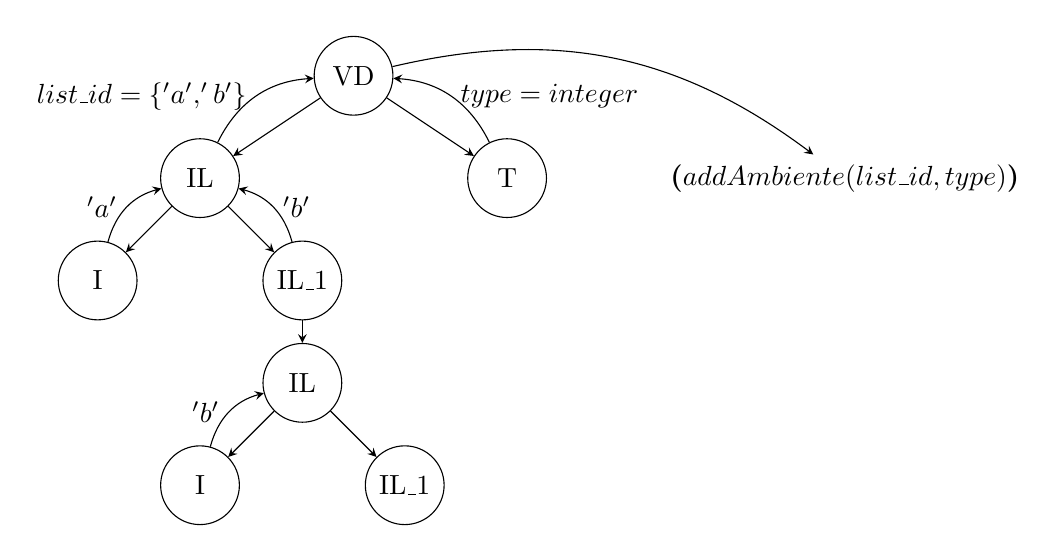
\begin{tikzpicture}[scale=0.65, node distance = 2.5cm, state/.style={circle, draw, minimum size=1cm}]
\tikzset{every state/.append style={thick, fill=gray!10}}
\node[state] (0) at (0,6) {VD};
\node[state] (1) at (-3,4) {IL};
\node[state] (2) at (3,4) {T};
\node[state] (3) at (-1,2) {IL\_1};
\node[state] (4) at (-5,2) {I};
\node[state] (5) at (-1,0) {IL};
\node[state] (6) at (1,-2) {IL\_1};
\node[state] (7) at (-3,-2) {I};

\node[right] (8) at (6,4) {{\bf ($addAmbiente(list\_id, type)$)}};

\path[->,>=stealth]
(0) edge[above] node{$ $} (1)
    edge[above] node{$ $} (2)
    edge[bend left=25] node{$ $} (8)

(1) edge[above] node{$ $} (3)
    edge[above] node{$ $} (4)
    edge[bend left, left] node{$list\_id=\{'a','b'\}$} (0)

(2) edge[bend right, right] node{$type=integer$} (0)

(3) edge[bend right, right] node{$'b'$} (1)
    edge[above] node{$ $} (5)
    
(4) edge[bend left, left] node{$'a'$} (1)

(5) edge[above] node{$ $} (6)
    edge[above] node{$ $} (7)

(7) edge[bend left, left] node{$'b'$} (5)
   % edge[bend left, left] node{$ $} (3)
;
\end{tikzpicture}
\caption{Declaración simple de variables.}
\label{fig:arbol_declaracion_var}
\end{figure}

En la figura \ref{fig:arbol_declaracion_var} se ve un árbol de derivación anotado teniendo en cuenta la gramática de atributos  y el uso de la tabla de símbolos, para la definición de dos variables integer: ``VAR a,b:integer;''. Cuando el no terminal VD obtiene el atributo list\_id que tiene la lista de identificadores declarados y type que tiene el tipo de dato de los identificadores, puede insertarlos en el Ambiente actual, que representa la tabla de símbolos de la subrutina que está analizando.

\begin{figure}[H]
\centering
\begin{tikzpicture}
\tikzset{every state/.append style={thick, fill=gray!10}}
\node[state] (0) at (0,6) {VDL};
\node[state] (1) at (-2,4) {VD};
\node[state] (2) at (2,4) {VDL\_1};
\node[coordinate] at (-2,2) (3) {};
\node at (-2,2) [isosceles triangle, shape border rotate=+90,
draw,minimum size=8mm,minimum height=2cm,
anchor=north] (3triangle) { };
%Inserta a,b:integer como en el árbol de la fig. \ref{fig:arbol_declaracion_var}
\node[right] (5) at (-4,-0.5) {Inserta a,b:integer};
\node[right] (6) at (-4,-1) {como en el árbol de la fig. \ref{fig:arbol_declaracion_var}};

\node[state] (4) at (2,2) {VD};
\node[coordinate] at (2,0) (5) {};
\node at (2,0) [isosceles triangle, shape border rotate=+90,
draw,minimum size=8mm,minimum height=2cm,
anchor=north] (5triangle) { };
%Inserta c:boolean como en el árbol de la fig. \ref{fig:arbol_declaracion_var}
\node[right] (7) at (0,-2.5) {Inserta c:boolean};
\node[right] (8) at (0,-3) {como en el árbol de la fig. \ref{fig:arbol_declaracion_var}};

\path[->,>=stealth]
(0) edge[above] node{$ $} (1)
    edge[above] node{$ $} (2)

(1) edge[above] node{$ $} (3)

(2) edge[above] node{$ $} (4)

(4) edge[above] node{$ $} (5)
;
\end{tikzpicture}
\caption{Declaración de listas de variables.}
\label{fig:arbol_declaracion_list_var}
\end{figure}

En la figura \ref{fig:arbol_declaracion_list_var} se ve el árbol de derivación para insertar una lista de variables con la siguiente sintaxis: ``VAR a,b:integer; c:boolean''. Así, la subrutina que está siendo analizada va a recibir todas sus variables sin importar cómo sea la declaración de variables.

En el siguiente árbol de la figura \ref{fig:arbol_declaracion_param} veremos la declaración de un procedimiento con parámetros, similar a la declaración de variables pero jugando un poco más con la tabla de símbolos.

\begin{figure}[H]
	\centering
	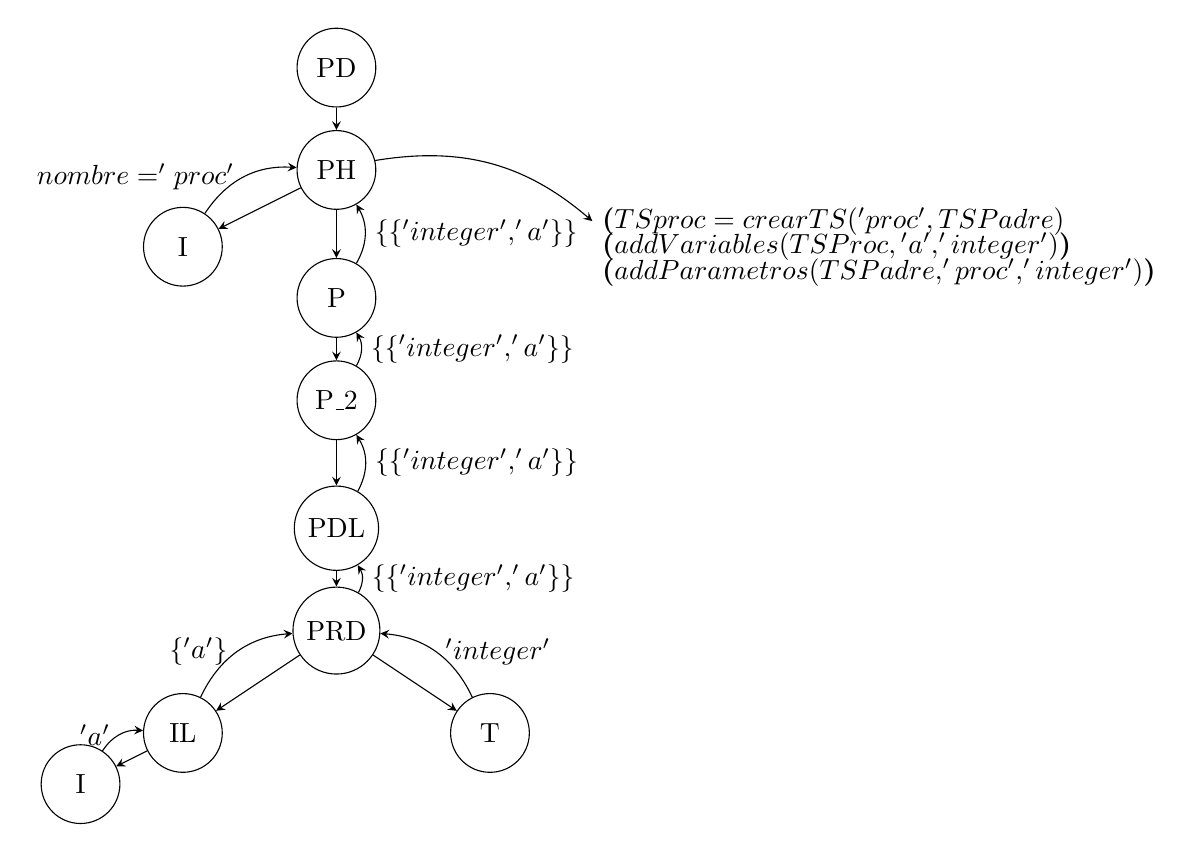
\begin{tikzpicture}[scale=0.65, node distance = 2.5cm, state/.style={circle, draw, minimum size=1cm}]
	\tikzset{every state/.append style={thick, fill=gray!10}}
	\node[state] (0) at (0,6) {PD};
	\node[state] (1) at (0,4) {PH};
	\node[state] (2) at (-3,2.5) {I};
	\node[state] (3) at (0,1.5) {P};
	\node[state] (4) at (0,-0.5) {P\_2};
	\node[state] (5) at (0,-3) {PDL};
	\node[state] (6) at (0,-5) {PRD};
	\node[state] (7) at (-3,-7) {IL};
	\node[state] (8) at (3,-7) {T};
	\node[state] (9) at (-5,-8) {I};	
	
	\node[coordinate] at (5,3) (InsTS) {};
	\node[right] (10) at (5,3) {{\bf ($TSproc = crearTS('proc',TSPadre)$}};
	\node[right] (11) at (5,2.5) {{\bf ($addVariables(TSProc,{'a'}, 'integer')$)}};
	\node[right] (12) at (5,2) {{\bf ($addParametros(TSPadre,'proc', 'integer')$)}};
	
	\path[->,>=stealth]
	(0) edge[above] node{$ $} (1)
	
	(1) edge[above] node{$ $} (2)
	edge[above] node{$ $} (3)
	edge[bend left=25] node{$ $} (InsTS)
	
	(2) edge[bend left, left] node{$nombre='proc'$} (1)
	
	(3) edge[above] node{$ $} (4)
	edge[bend right, right] node{$\{\{'integer','a'\}\}$} (1)
	
	(4) edge[bend right, right] node{$\{\{'integer','a'\}\}$} (3)
	edge[above] node{$ $} (5)
	
	(5) edge[above] node{$ $} (6)
	edge[bend right, right] node{$\{\{'integer','a'\}\}$} (4)
	
	(6) edge[above] node{$ $} (7)
	edge[above] node{$ $} (8)
	edge[bend right, right] node{$\{\{'integer','a'\}\}$} (5)
	
	(7) edge[above] node{$ $} (9)
	 edge[bend left, left] node{$\{'a'\}$} (6)
	 
	(8) edge[bend right, right] node{$'integer'$} (6)
	 
	(9) edge[bend left, left] node{$'a'$} (7)
	% edge[bend left, left] node{$ $} (3)
	;
	\end{tikzpicture}
	\caption{Declaración simple de variables.}
	\label{fig:arbol_declaracion_param}
\end{figure}

En la figura \ref{fig:arbol_declaracion_param} se muestra el análisis para la declaración del encabezado de un procedimiento con la sintaxis: ``procedure proc(a:integer);''. El árbol muestra cómo se obtiene el nombre del procedimiento, sus parámetros y luego en el nodo PH se procede a crear la nueva tabla de símbolos para ese procedimiento, la cual recibe como parámetro el nombre del procedimiento y la tabla de símbolos del padre (teniendo en cuenta su estructura lexicográfica). Luego se agregan los parámetros como variables a la tabla del procedimiento; y se agregan los tipos de los parámetros a la tabla del procedimiento padre, para que cuando se invoque a \emph{proc}, pueda chequear la cantidad y el tipo de los parámetros que se le envían.

Si la declaración de parámetros fuera la siguiente: (a,b:integer;c:boolean), en el nodo PRD se armaría la siguiente lista: \{\{'integer','a','b'\},\{'boolean','c'\}\}, y una vez que llegue a PH se ejecutaría \\ 
addVariables(TSProc,'a','integer'), addVariables(TSProc,'b','integer'), addVariables(TSProc,'c','boolean') y \\ addParametros(TSPadre,'proc',\{'integer','integer','boolean'\}). 

\subsection{Instructivos de instalación y uso}
Para usar el programa es idéntico que para el Análizador Sintáctico, al ser un programa portable, solo se requiere la compilación a través del comando \emph{javac *.java} o cargando el proyecto en el NetBeans y usando este para compilar.

Para ejecutar, hay que invocar el programa compilado enviándole como parámetro el archivo con el código fuente del programa a compilar.

También es posible ejecutar la batería de ejemplos mediante el ejecutable \texttt{bateria-wind.bat} para Windows o \texttt{bateria-linux.sh} para Linux.

\subsection{Ejemplos}
Para mostrar el funcionamiento del Analizador Semántico proponemos una serie de ejemplos para demostrar las funcionalidades semánticas implementadas.

%unicidad
\subsubsection{Chequeo de unicidad}
\begin{figure}[H]
\begin{minted}[escapeinside=||,autogobble,linenos,xleftmargin=0.35\textwidth,xrightmargin=0.35\textwidth]{pascal}
Program Example1;
Var       
    Num1, Num2, Sum1 : Integer;
    |!Num1!|: Boolean;
Begin
    Sum := Num1 + Num2;
    if (Num1 > Num2) then
        Result := true
End.
\end{minted}
\caption{Programa en Pascal reducido con error de unicidad en variable Num1.}
\label{fig:semantico_ej_error_1}
\end{figure}

\begin{figure}[H]
\centering
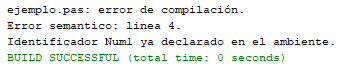
\includegraphics[]{img/semantico/semantico_ej1.png}
\caption{Resultado compilación ejemplo1.}
\label{fig:semantico_ej1}
\end{figure}

%existencia \(declaración de variable\)
\subsubsection{Chequeo de existencia}
\begin{figure}[H]
\begin{minted}[escapeinside=||,autogobble,linenos,xleftmargin=0.35\textwidth,xrightmargin=0.35\textwidth]{pascal}
Program Example2;
Var       
    Num1, Num2, Sum1 : Integer;
Begin 
    Num1 := 2;
    |!Sum2!| := Num1 + Num2;
End.
\end{minted}
\caption{Programa en Pascal reducido con falta de declaración de variable Sum2.}
\label{fig:semantico_ej_error_2}
\end{figure}

\begin{figure}[H]
\centering
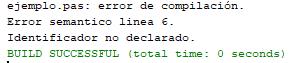
\includegraphics[]{img/semantico/semantico_ej2.png}
\caption{Resultado compilación ejemplo2.}
\label{fig:semantico_ej2}
\end{figure}

%correspondencia de parametros en llamada a funcion
\subsubsection{Correspondencia de parámetros}
\begin{figure}[H]
\begin{minted}[escapeinside=||,autogobble,linenos,xleftmargin=0.35\textwidth,xrightmargin=0.35\textwidth]{pascal}
Program Example3;
Var       
    Num1, Num2, Sum1 : Integer;
    Procedure proc(a:integer, b:boolean);
    begin
        b := true;
    end;
Begin
    proc(Num1,true);
    |!proc(Num1,Num2)!|
End.
\end{minted}
\caption{Programa en Pascal reducido con error en la llamada al procedimiento proc en la línea 10.}
\label{fig:semantico_ej_error_3}
\end{figure}

\begin{figure}[H]
\centering
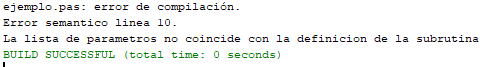
\includegraphics[]{img/semantico/semantico_ej3.png}
\caption{Resultado compilación ejemplo3.}
\label{fig:semantico_ej3}
\end{figure}

%uso de identificador funcion para devolver su resultado 
\subsubsection{Devolver valor de una función}
\begin{figure}[H]
\begin{minted}[escapeinside=||,autogobble,linenos,xleftmargin=0.35\textwidth,xrightmargin=0.35\textwidth]{pascal}
Program Example4;
Var       
    Num1, Num2, Sum1 : integer;
    function f1(a:integer): integer ;
    begin
        |!f1!| := a+3;
    end;
Begin
    f1(Num1)
End.
\end{minted}
\caption{Programa en Pascal reducido con uso de identificador f1 para devolver un valor.}
\label{fig:semantico_ej_error_4}
\end{figure}

\begin{figure}[H]
\centering
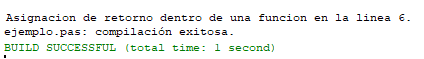
\includegraphics[]{img/semantico/semantico_ej4.png}
\caption{Resultado compilación ejemplo4.}
\label{fig:semantico_ej4}
\end{figure}

%compatibilidad de tipos para asignacion
\subsubsection{Compatibilidad de tipos}

\begin{figure}[H]
\begin{minted}[escapeinside=||,autogobble,linenos,xleftmargin=0.35\textwidth,xrightmargin=0.35\textwidth]{pascal}
Program Example5;
Var       
    Num1, Num2, Sum1 : Integer;
    Procedure proc(a:integer, b:boolean);
    begin
        a := 3;
        |!b := a;!|
    end;
Begin
    proc(Num1,Num2)
End.
\end{minted}
\caption{Programa en Pascal reducido con error en la compatibilidad de tipos línea 7.}
\label{fig:semantico_ej_error_5}
\end{figure}

\begin{figure}[H]
\centering
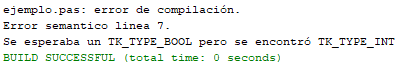
\includegraphics[]{img/semantico/semantico_ej5.png}
\caption{Resultado compilación ejemplo5.}
\label{fig:semantico_ej5}
\end{figure}

%\section{Problemas encontrados}
%ni ahi

%\section{Posibles mejoras}
%ninguna

\section{Conclusión}
Cumplimos con los requerimientos propuestos en la descripción del problema \ref{sec:sem:descr_probl}, extendiendo el Analizador Sintáctico con las reglas semánticas y utilizando los atributos descritos en \ref{sec:sem:gram_atrib}. 
